\documentclass[letterpaper,10pt]{article}

\usepackage{titling}
\usepackage{listings}
\usepackage{url}
\usepackage{setspace}
\usepackage{subfig}
\usepackage{sectsty}
\usepackage{pdfpages}
\usepackage{colortbl}
\usepackage{multirow}
\usepackage{relsize}
\usepackage{amsmath}
\usepackage{fancyvrb}
\usepackage{amsmath,amssymb,amsthm,graphicx,xspace}
\usepackage[titlenotnumbered,noend,noline]{algorithm2e}
\usepackage[compact]{titlesec}
\usepackage[default]{droidserif}
\usepackage[T1]{fontenc}
\usepackage{tikz}
\usetikzlibrary{arrows,automata,shapes,trees,matrix,chains,scopes,positioning,calc}
\tikzstyle{block} = [rectangle, draw, fill=blue!20, 
    text width=2.5em, text centered, rounded corners, minimum height=2em]
\tikzstyle{bw} = [rectangle, draw, fill=blue!20, 
    text width=4em, text centered, rounded corners, minimum height=2em]

\definecolor{namerow}{cmyk}{.40,.40,.40,.40}
\definecolor{namecol}{cmyk}{.40,.40,.40,.40}

\let\LaTeXtitle\title
\renewcommand{\title}[1]{\LaTeXtitle{\textsf{#1}}}


\newcommand{\handout}[5]{
  \noindent
  \begin{center}
  \framebox{
    \vbox{
      \hbox to 5.78in { {\bf ECE155: Engineering Design with Embedded Systems } \hfill #2 }
      \vspace{4mm}
      \hbox to 5.78in { {\Large \hfill #4  \hfill} }
      \vspace{2mm}
      \hbox to 5.78in { {\em #3 \hfill} }
    }
  }
  \end{center}
  \vspace*{4mm}
}

\newcommand{\lecture}[3]{\handout{#1}{#2}{#3}{Lecture #1}}
\newcommand{\tuple}[1]{\ensuremath{\left\langle #1 \right\rangle}\xspace}

\addtolength{\oddsidemargin}{-1.000in}
\addtolength{\evensidemargin}{-0.500in}
\addtolength{\textwidth}{2.0in}
\addtolength{\topmargin}{-1.000in}
\addtolength{\textheight}{1.75in}
\addtolength{\parskip}{\baselineskip}
\setlength{\parindent}{0in}
\renewcommand{\baselinestretch}{1.5}
\newcommand{\term}{Spring 2014}

\singlespace

\DeclareUrlCommand\j{}

\begin{document}

\lecture{ 29 --- Software Statistics}{\term}{Eric David Hollbach \& Mahesh Tripunitara, edited by Jeff Zarnett}

\section*{The Setting}\label{sec:setting}
The Java SDK \cite{java:set} specifies an interface called \j{Set}. Its semantics
is the mathematical notion of a set --- an unordered collection of unique items. You can have a set of integers like \{ 8, 16, 44, 18, 99, -1 \}, but duplicates are not permitted in a set.
Several implementations of \j{Set} are provided by the SDK. Are they all the same? If not, which one should we use?

They are not identical, so we expect that the answer is: ``it depends on your application.'' However, it is reasonable to expect that there exist some criteria to which we should
be able to agree based on which we compare different implementations of \j{Set}.
We want these two operations to be fast:
\begin{enumerate}
    \item Addition (putting something in the set); and
    \item Membership-checking (finding out if an element is a member of the set) to be fast.
\end{enumerate}

These criteria, in turn, provide an objective way of evaluating if
one implementation is better than another. Thus, our goal is
more modest than the absolute, non-comparative, criterion of ``fast''. 
We are just figuring out if one set-implementation
is ``better than'' (faster than) another in these two operations.

The question now is: how can we evaluate two given implementations in a rigorous and consistent way?

\section*{Statistics} \label{sec:statistics}

We use statistics to try to establish that (if?) one set-implementation
is better than another. The application of statistics 
to this question is not straightforward. To illustrate this via
an example, consider a scenario where Alice follows the process below:

\begin{enumerate}
\item Randomly choose a bunch of integers (let's say 100).

\item Use some API for measuring time on the computer.
Write Java code to measure the time it takes to add each of
those integers to an instance of a set-implementation $I_1$,
starting at $I_1 = \emptyset$ (the empty set). Compute the average time, $a_1$.

\item Repeat for an instance of another set-implementation
$I_2$ to get the average $a_2$ for it.

\item If $a_1 < a_2$, conclude that the first set-implementation
is better than the second from the standpoint of additions to the set.
\end{enumerate}

What is wrong with adopting the above process?

\begin{enumerate}
    \item How do we know that the random set of integers Alice chooses
	is representative of all possible integers we may want to
	add to a set?
    \item Do we have to consider the order in which we add
	the integers? For example, starting with a set $S$, it
	is possible that adding integer $i_1$ then $i_2$ may
	result in a different total time for the two additions
	than adding $i_2$ and then $i_1$.
    \item Why is it meaningful to use the average to draw our
	conclusion?
    \item Even if we feel that use of the average is meaningful,
	how do we know that the averages are \emph{statistically
	significant}? That is, how do we know that we can make a
	conclusion based on the fact that $a_1 < a_2$? Is it possible
	that in a run of this experiment, we ended up with
	$a_1 < a_2$ purely by chance?
    \item Computers demonstrate considerable variations over
	time in how long they take to perform an operation. That is,
	if you run the Java code again, the time for adding a 
	particular integer $i$ to the set in the second run may
	result in a different time-measurement than the first time.
	How do we know that we can trust the reading which contributes
	to the average based on which we draw our conclusion?
\end{enumerate}

Ideally, we will have good answers to all of the above questions.
Even if we are unable to conclusively address a concern such
as the above, it is very important to recognize the concern. And
at the minimum articulate an assumption explicitly.

\subsection*{Basics} \label{sec:statistics:basics}
A (mathematical) \emph{function} is defined as follows. Given two sets,
a domain and a range, a function associates a member of the
range with every member of the domain.

We can associate the time it takes to add or membership-check
an element against a set as a \emph{random variable}.
A random variable is a function
$f\!\! : E \longrightarrow \mathbb{R}$, where $E$ is a set
of \emph{events}, and $\mathbb{R}$ is the set of 
real numbers. In our case, the range of a random variable
we choose is presumably the time it takes to add
the item to the set, or check its membership in the set.
We choose the domain based on the assumptions we make.
For this work, we choose the domain $E$ as the set
of all integers.

That is, we adopt two random variables, $a, m$, the former
for add and the latter for membership-checking. Each maps
an integer to a time-value. One of the points of characterizing
$a, m$ as random variables is that
we typically associate
a random variable with a \emph{probability distribution}.

A probability distribution is itself a function. It maps
each event in $E$ to a probability that it occurs.
For example, it is possible that the
probability that we add the integer $15$ to a set,
is different from the probability that we add $32$.
Thus, the probability we associate with the event
$\tuple{15}$ is different from the probability
we associate with the event $\tuple{32}$.

If we can discover this $a(e)$ and $m(e)$
for a ``typical'' $e \in E$ for
two different set-implementations, then we can draw a conclusion.
This has two challenges: (1) what is a ``typical'' $e \in E$, and,
(2) how do we compute $a$ and $m$ even if we know this $e$?

\subsection*{Characterizing $a$ and $m$}\label{sec:statictics:charac}
The domain of a random variable ($E$, above) is called a
\emph{population}. To characterize a random variable, an approach
is to determine to what value in the range it maps every member of
the population, and then compute a \emph{central tendency} or
\emph{centre} of those values.
A centre, as its name suggests, represents the ``middle'' of
all possible values. The \emph{average}, the sum of all values
divided by the number of values, is a centre. Other examples of
centres are the \emph{median} and \emph{trimean}.
The choice of a centre is crucial. Not every centre is
\emph{robust} to \emph{outliers}. An outlier is a value
that occurs infrequently. Robustness is the property that
a centre is representative of the ``middle'' notwithstanding
the presence of outliers. We discuss further our choice
of the centre below.

It is often impractical or even impossible to compute a
centre for the entire population. For example, if the population
is all Canadians, determining the value of a random variable
for every Canadian may be deemed too expensive.
Consequently, we collect data \emph{samples}.
A sample is a particular member of the population.
The procedure by which we collect samples is important. Otherwise,
the samples may not reflect the properties of the population,
and thereby, the random variable.

Given a random variable $X$ whose underlying
probability distribution is $P$, a well-accepted property of
samples is that they are: (1) \emph{independent and identically
distributed} (iid), and, (2) each sample, when viewed as a
random variable
in its own right, has the same distribution $P$ as $X$.

With regards to (1),
a set of random variables is said to be iid if each random
variable from the set has the same probability distribution
as all the other random variables in the set.
With regards to (2), as an example,
if $X$ is the random variable that is the height
of a person, then the manner in which we collect samples must
reflect the distribution of heights amongst individuals.
If the probability that there exists a person of height $h$ in
the entire population is $\rho$, then the probability that height
$h$ ends up in our set of samples must be $\rho$.
(Or, the probability that we pick a person of height $h$ to be
part of our sample-set must be $\rho$.)

We now address three issues we must resolve: how do we choose
a sample, what is our choice for centre, and how do we compute
our choice of centre for the random variables $a,m$ given the
samples we choose?

\paragraph{Choice of samples} Our discussions above indicate that
we should choose samples in a manner that reflects the population.
A difficulty for us is that we do not know what the underlying
distribution of integers in the population is.
That is, we do not know what kinds of 
integers are added/membership-checked
in them. We resolve this issue by assumption.

We would of course like to minimize the number and nature of
assumptions in any study. However, practicality may require that
we make some. And it is okay to make assumptions, provided
we clearly state them, and remember them when the time comes to draw conclusions.
%This is a very important part
%of being an objective techie --- being clear and open about any
%assumptions that are made in an analysis.

We have done the following in our study.
We have restricted ourselves to integer items only.
We make the assumption that every integer is
equally likely to be added to, or queried for, in a set.
This restriction and assumption limits the applicability
of our results. So, one needs to be careful in applying or
interpreting our results.

\paragraph{Choice of centre} Our choice of centre is the
average, or mean. We choose this for convenience --- it is
easy to compute an average, particularly for a continuous
(i.e., non-discrete) values.

The mean is not \emph{robust} against outliers.
An outlier is an atypical value, that is, a value that occurs
with low probability. An outlier can skew the mean in a manner
that the mean is no longer a meaningful centre.
The median, on the other hand, is robust.
The median of a continuous random variable is a value, $m$,
such that the probability that a given value lies above
or below $m$ is $1/2$.

In our hypothesis testing below, we assume that the population
is distributed normally. In such a case, the mean and median
are the same. Note that it is possible to test for normality,
rather than simply assume it. We omit a discussion of that, and
urge you to take a stats course. Statistics is a big and complex
subject and easily takes up a whole course all on its own.

\paragraph{Computing the centre for $a, m$} Given our above
assumptions, to compute the centre (average, in our case), we
simply pick random integers to add/query, check how long it
takes, and compute the average for some large number of such
trials.

There are some additional issues we need to consider, however.

\begin{itemize}
    \item The time for individual additions/queries can be
	so small that the measurement mechanism we use can
	be highly unreliable. We resolve this by performing
	several adds/queries, and measuring the time for those.
	We have chosen 250,000 adds/queries.

    \item Java VMs demonstrate strange behaviour when running
	such experiments. Specifically, there is a ``warm up''
	period for every VM after it starts to run
	that we need to exclude.

	A way that has been proposed to deal with this \cite{xxx}
	is to measure a statistic called the coefficient
	of variance (CoV) across some number, call it
	$k$, of measurements. Then, check whether this
	CoV is below some threshold. This approach is
	supposedly robust in practice.

	We have also run our experiments several times, across
	several days and times of the day. And established that
	there is no statistically significant variance across
	those.
\end{itemize}

\subsection*{Hypothesis Testing}\label{sec:statistics:hypo}
Now that we have decided on a centre and how to compute it,
we can compare the three implementations of set across
each of the two axes, add-time and query-time.
We do this by comparing two implementations at a time.
Given two implementations, say, \texttt{TreeSet} and \texttt{HashSet},
we ask whether the difference in the centres for them
is statistically significant. An effective way to establish
this is via a hypothesis test.

In a hypothesis test, we articulate a hypothesis, that is,
an assertion that may be true or false. We then ask whether
the hypothesis should be accepted or rejected. In statistics,
we typically enunciate a \emph{null hypothesis}.
It is called that because it is usually a hypothesis of
`no effect,' or `no difference.' In our case, an appropriate
null hypothesis is that there is no difference in performance
between two different implementations of set.

The complement of the null hypothesis is called an
\emph{alternate hypothesis}.
If we articulate a null hypothesis as above, then the alternate
hypothesis is that there is a difference in performance
between \texttt{HashSet} and \texttt{TreeSet}.

It is important to point out that our null hypothesis was posed
before we designed the statistical experiments. Posing hypotheses
after looking at data is dangerous, as it 
can compromise objectivity and lead to incorrect inferences. As
Sherlock Holmes said, it's unwise to form the theory before getting the facts;
we have a tendency to twist the facts to fit the theory when we should
be using the facts to generate the theory.

Once we choose a null hypothesis,
we choose a probability $p$ which is the threshold at which
we \emph{reject} the null hypothesis and adopt the alternate
hypothesis. The meaning of a value for $p$ is:
\begin{quote}
    If the null hypothesis is true, then
    there is a probability $p$ of observing a difference
    in the averages as large as we observe.
\end{quote}

As you can tell from the above semantics for $p$, a smaller
value for $p$ as threshold is better, i.e., suggests more
statistical significance. This is because if the null hypothesis
is indeed true, then there is only a small chance of observing
the difference in averages that we did observe. Therefore,
the fact that we did observe it, and can presumably reproduce
the observations if we repeat the experiment, suggests that
probabilistically, the null hypothesis is false.

\begin{center}
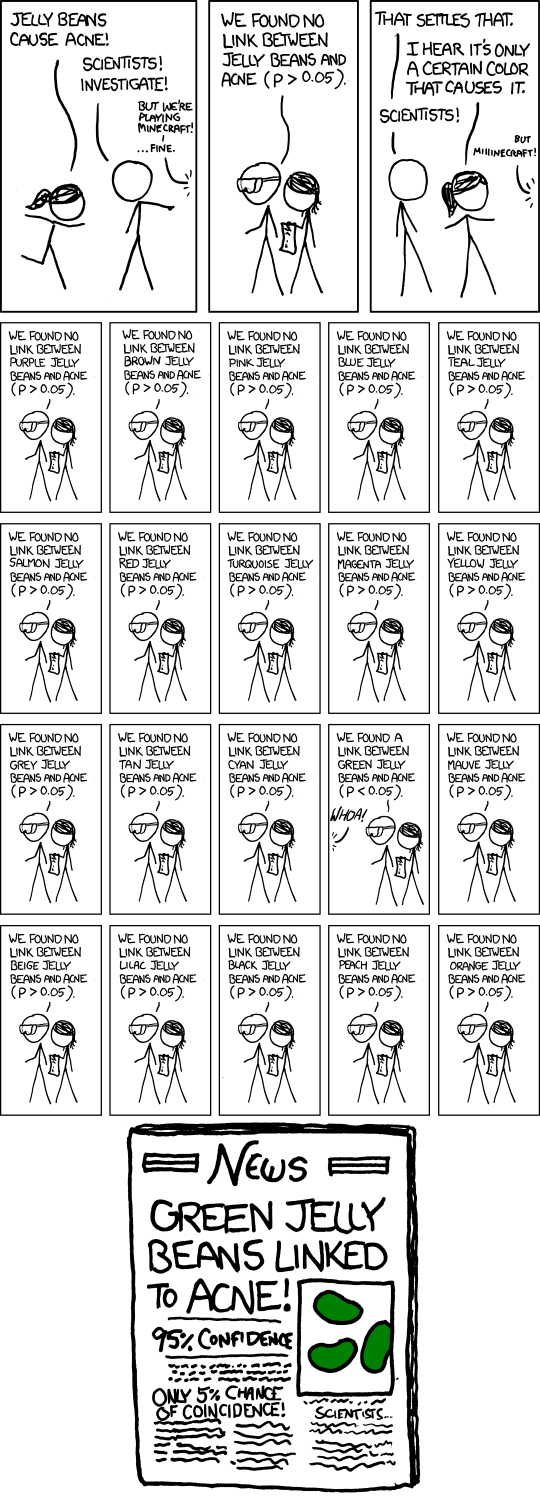
\includegraphics[width=0.5\textwidth]{images/significant.png}~\cite{xkcd:significance}
\end{center}

\paragraph{Choice of test} There are a number of tests from
which one could choose. The main thing to note here is the
prerequisites each tests requires for it to be sound.
For example, a number of tests require that the underlying
population is distributed normally.

We do not go over the fundamentals of particular tests. You
should take a course on statistics for that. But we again
warn you that before you use any particular test, you should
carefully read about the pre-conditions for the test to be
applicable. For example, we use the Student's t-test in
our following discussion. 

The requirements for the Student's t-test in our context
are: (1) the data is continuous, (2) the data follows a normal
probability distribution, (3) the samples are independent, and
(4) they are simple random samples from the respective populations.
We know that (1) is true if we assume that any value for time may
occur, and we ensure (3) and (4) from the
manner in which we choose the samples. We satisfy (2) by
assumption.

\paragraph{Results} Following are the average and standard
deviation, in seconds, for \texttt{HashSet}, \texttt{LinkedHashSet }
and \texttt{TreeSet} for
adding 250,000 integers starting from the empty set.
\begin{center}
    \begin{tabular}{l|c|c}
	\textbf{Implementation} & \textbf{Average} & \textbf{Std.~Dev.}\\ \hline
	\texttt{HashSet} & $0.183095$ & $0.00124$ \\ \hline
	\texttt{LinkedHashSet} & $0.20011$ & $0.000609$ \\ \hline
	\texttt{TreeSet} & $0.3975$ & $0.00222$ \\
    \end{tabular}
\end{center}

Following are the average and standard
deviation, in seconds, for \texttt{HashSet}, 
\texttt{LinkedHashSet} and \texttt{TreeSet} for
querying each of the 250,000 integers that have been added.
Thus, our queries are elements we know to be in the set only.
We articulate our null hypothesis accordingly to account for
not testing for elements that are not in the set.
\begin{center}
    \begin{tabular}{l|c|c}
	
	\textbf{Implementation} & \textbf{Average} & \textbf{Std.~Dev.}\\ \hline
	\texttt{HashSet} & $0.029934$ & $0.000685$ \\ \hline
	\texttt{LinkedHashSet} & $0.083366$ & $0.001148$ \\ \hline
	\texttt{TreeSet} & $0.097701$ & $0.002612$ \\
    \end{tabular}
\end{center}

In reporting such numbers, it is important to identify as much
of the setup as possible so there is sufficient information
for someone to reproduce these results. Our information is:

\begin{quote}
 the experiments were conducted on an isolated Intel dual core
 ASUS P5LD2-VM PC with a 3 GHz processor and 3.1 GiB of RAM,
 running the Ubuntu Linux operating system. The java
 version was 1.6.0\_31, and it was the OpenJDK Runtime Environment.
 To measure time, we used System.nanoTime().
 Each of our averages are over 30 iterations after the VM
 reached steady-state.
 \end{quote}
 Steady-state refers to the VM after 
 warm-up. See our discussions above under,
 `Computing the centre\ldots'

\paragraph{Hypothesis tests} We now articulate null hypothesis,
and a choice for the threshold $p$ value, and conduct our tests.
As an example, we have chosen a two-tailed, unpaired
Student's t-test. Again, we urge you to take a stats course
to understand the test in more depth. We have used 
GraphPad's QuickCalcs site, \url{http://www.graphpad.com/quickcalcs/},
to enter our data and run the tests.

As $p$ value, we choose, say, $0.01$, i.e., $1\%$. This choice
is arbitrary, and really depends on what your peers will accept.
In conducting a hypothesis test in the context of the discovery
of Higgs Boson, for example, the $p$ value was chosen as
``five-sigma'' (i.e., $5$ times the standard deviation), which
corresponds to a $p$ threshold value of $3\times 10^{-7}$.
(See the discussion at \url{http://blogs.scientificamerican.com/observations/2012/07/17/five-sigmawhats-that/}.)

We choose a much more conservative threshold of $0.01$.
So, we reject the null hypothesis if the calculated probability
is less than $0.01$.

Our first null hypothesis is, ``To add 250,000 integers, there
is no difference in time between \texttt{HashSet} and \texttt{LinkedHashSet}.''
The Student's t-test run with our above mean, standard deviation
and $N$ (number of samples, which in our case is $30$) produces
the following output:
\begin{quote}
    The two-tailed P value is less than $0.0001$.
\end{quote}
That is, the computed probability is less than our threshold
probability of $0.01$. Therefore, we reject the null hypothesis
that there is no difference in performance. There is just one
more issue, however. Our alternate hypothesis is that there
is a difference in performance. But not that a particular one
of those is better than the other. However, we could informally
look at our data and conclude that our experiments suggest that
\texttt{HashSet} performs better than \texttt{LinkedHashSet}, given all our
assumptions and choices.

We can similarly perform the other two comparisons,
\texttt{HashSet} vs. \texttt{TreeSet}, and \texttt{LinkedHashSet}
 vs. \texttt{TreeSet}, and get
similar results. Similarly, a Student's t-test for the
null hypothesis, ``there is no difference in querying 250,000
members of \texttt{LinkedHashSet} and \texttt{TreeSet}'' using our data from
the table above for querying produces the same output as above:
\begin{quote}
    The two-tailed P value is less than $0.0001$.
\end{quote}

\paragraph{Multiple comparisons} Are we done? Unfortunately, not
quite. In the above, we have performed a pairwise comparison
of three groups. This is an example of a situation that makes
us susceptible to a problem known as \emph{multiple comparisons}.
The problem is that we posed multiple hypotheses using the same
data. Therefore, the chance that we see statistical significance
in some pairwise comparison is increased purely by chance.

Consider our situation, in which we have only a probability of
$0.01$ of erroneously rejecting each null hypothesis if indeed
the null hypothesis is true. We have, however, posed three
such hypotheses. Therefore,
$\text{Pr}\{\ge 1 \text{ erroneous rejection}\} =
1 - \text{Pr}\{\text{no erroneous rejection}\} =
1 - (0.99)^3 \approx 0.03 > 0.01$. (We multiply the three
probabilities, $0.99$, under the assumption that those
probabilities across the three tests are independent.)

How do we address this? A natural way is to correct
for the multiple comparisons. A correction is suggested
by the example above, and is called the Bonferroni
correction. Under the Bonferroni correction, to test
$k$ hypotheses with a desired significance level of
$s$, we test each hypothesis at a significance level
of $s/k$. In our case, $k=3$, and so we need to test
each of our pairwise hypotheses at a threshold of
$0.0033$ so that the family of tests has a threshold
of $0.01$.

In our case, the computed probability
based on the data is less than $0.0033$ for each test,
so our conclusions are remain valid.

The Bonferroni correction is conservative, i.e.,
overkill, and therefore safe. A more exact
correction can be applied instead. The way we computed the
probability above for erroneously rejecting at least
one null hypothesis is the way to compute an exact
correction, but we omit the details.

\paragraph{Closing}
This is just an introduction to the use of statistics in evaluating
software performance. The techniques are sound but this is a complicated
subject and the brief overview in this lecture is by no means a substitute
for a full course on statistics. However, it should serve to alert you
to the issues and perhaps whet your appetite to investigate such matters
further in the future. 

\bibliographystyle{alpha}
\bibliography{155}


\end{document}
